\documentclass{article}


% if you need to pass options to natbib, use, e.g.:
% \PassOptionsToPackage{numbers, compress}{natbib}
% before loading nips_2018

% ready for submission
% \usepackage{nips_2018}

% to compile a preprint version, e.g., for submission to arXiv, add
% add the [preprint] option:
\usepackage[final]{nips_2018}

% to compile a camera-ready version, add the [final] option, e.g.:
% \usepackage[final]{nips_2018}

% to avoid loading the natbib package, add option nonatbib:
% \usepackage[nonatbib]{nips_2018}

\usepackage[utf8]{inputenc} % allow utf-8 input
\usepackage[T1]{fontenc}    % use 8-bit T1 fonts
\usepackage{hyperref}       % hyperlinks
\usepackage{url}            % simple URL typesetting
\usepackage{booktabs}       % professional-quality tables
\usepackage{amsfonts}       % blackboard math symbols
\usepackage{amsmath}
\usepackage{nicefrac}       % compact symbols for 1/2, etc.
\usepackage{microtype}      % microtypography
\usepackage[pdftex]{graphicx}
\graphicspath{ {images/} }



\title{Recurrent Neural Networks for Time Series Prediction}

% The \author macro works with any number of authors. There are two
% commands used to separate the names and addresses of multiple
% authors: \And and \AND.
%
% Using \And between authors leaves it to LaTeX to determine where to
% break the lines. Using \AND forces a line break at that point. So,
% if LaTeX puts 3 of 4 authors names on the first line, and the last
% on the second line, try using \AND instead of \And before the third
% author name.

\author{
  Davide Spallaccini\thanks{\texttt{spallaccini.1642557@studenti.uniroma1.it}}
\\
  Department of Computer, Control \\ and Management Engineering\\
  Sapienza University of Rome\\
  Rome, Italy \\
  \And
  Beatrice Bevilacqua\thanks{\texttt{bevilacqua.1645689@studenti.uniroma1.it}}
\\
  Department of Computer, Control \\ and Management Engineering\\
  Sapienza University of Rome\\
  Rome, Italy \\
   \\
  %% examples of more authors
  \And
  Anxhelo Xhebraj\thanks{\texttt{xhebraj.1643777@studenti.uniroma1.it}} \\
  Department of Computer, Control \\ and Management Engineering\\
  Sapienza University of Rome\\
  Rome, Italy
  %% Affiliation \\
  %% Address \\
  %% \texttt{email} \\
  %% \AND
  %% Coauthor \\
  %% Affiliation \\
  %% Address \\
  %% \texttt{email} \\
  %% \And
  %% Coauthor \\
  %% Affiliation \\
  %% Address \\
  %% \texttt{email} \\
  %% \And
  %% Coauthor \\
  %% Affiliation \\
  %% Address \\
  %% \texttt{email} \\
}

\begin{document}
% \nipsfinalcopy is no longer used

\maketitle

\begin{abstract}

TODO

\end{abstract}

\section{Introduction and Related Work}
\label{sec:intro}

We will face the problem of time series prediction through Nonlinear
autoregressive exogenous models (NARX) whose
purpose is to predict the current value of a time series based on it's
collected knowledge coming from the history of
the time series to predict and the current and past values of a set of
exogenous time series. Exogenous time series
are data that may be correlated to the series under consideration so they are
also called "driving series". Of course
a good NARX algorithm should be able to choose which of the series are to be
considered "driving" when predicting the
current value. At the same time a good algorithm should be able to capture
long-term temporal dependencies.

In this work we analyse a deep-learning-based model that tries to takle with
these two issues through the use of
recurrent neural networks and a carefully combined system of attention
mechanisms. We also compare the result with
other possible approaches to the same problem using again recurrent networks
and also perform an ablation study that
wasn't directly reported in the author's paper to validate the effectiveness of
the approach proposed.

Models from the past, though effective for some real word applications, do not
perform very well since they cannot
model nonlinear relationships and do not differentiate beween driving terms, or
they model nonlinear relationships
but with a predefined nonlinear relationship which is not necessary the true
underlying one.

\section{Dataset}
\label{sec:retrieval}

We used the same dataset as the authors in order to try to compare our results
with the ones obtained by them. However
since the paper doesn't mention anything about data normalisation, selection or
other kinds of preprocessing we didn't
get their exact results. We still got results that we could use to compare the
different approaches and validate the
effectiveness of the use of the dual-stage attention mechanism.

The first dataset is SML 2010 is used to predict the temperature of indoor 
environments. The data is collected from sensors of a system mounted in a 
domestic house for a total time of 40 days. The data is sampled every minute and 
was smoothed with 15 minutes mean. The target series we select is the room 
temperature and we collect 16 driving series. Examples of driving series are: ...

The second one is the NASDAQ 100 Stock dataset which is characterised by a
larger number of driving series. This dataset is made public by the same authors of the original paper and is a collection of prices of 81 major corporations under NASDAQ 100 used as driving time series. The target series used is the value of the NASDAQ 100 index. As in the first dataset data is sampled every minute and covers 105 days from 26/07/2016 to 22/12/2016.

\section{Model}
\label{sec:model}

\subsection{Model definitions}
\paragraph{Dual-stage attention model}

The proposed model in our reference paper is composed of an input attention
whose output is fed to an encoder RNN. The
result is the input to a temporal attention and the output of this second
attention mechanism is composed with the
past history of the target time series to the decoder RNN. We notice that there
is a fixed-size interval of time from
which we sample a fixed number of timesteps ($T$ henceforward).

The input attention is trained to assign a weight to all the possible input
driving series. In particular we have
that each driving series is represented as a vector of $T$ values, one for each
timesteps. For each timestep $t$ the
input attention assigns a weight to each of the driving series values for that
timestep (i.e. at the offset $t$ of the
driving series vector).

The encoder RNN is implemented with a LSTM cell, this choice allows the model
to capture long-term dependencies.
For each timestep we map the result of the first attention to the output
$\mathbf{h}_t$ which is the hidden state of
the LSTM at timestep $t$. The operations involved in this mapping are the ones
that take place in the update of a LSTM
cell and can be summarised as follows:


\begin{equation} \label{eq:lstm}
\begin{split}
\mathbf{f}_t &= \sigma (\mathbf{W}_f[\mathbf{h}_{t-1};\mathbf{x}_t] +
\mathbf{b}_f) \\
\mathbf{i}_t &= \sigma (\mathbf{W}_i[\mathbf{h}_{t-1};\mathbf{x}_t] +
\mathbf{b}_i) \\
\mathbf{o}_t &= \sigma (\mathbf{W}_o[\mathbf{h}_{t-1};\mathbf{x}_t] +
\mathbf{b}_o) \\
\mathbf{s}_t &= \mathbf{f}_t \odot \mathbf{s}_t + \mathbf{i}_t 
				\odot
\text{tanh}(\mathbf{W}_s[\mathbf{h}_{t-1};\mathbf{x}_t] + \mathbf{b}_s) \\
\mathbf{h}_t &= \mathbf{o}_t \odot \text{tanh}(\mathbf{s}_t)
\end{split}
\end{equation}

Where $[\mathbf{h}_{t-1};\mathbf{x}_t] \in \mathbb{R}^{m + n}$ is a
concatenation of the hidden state of the previous
timestep and the input of the current timestep;
$\mathbf{W}_f,\mathbf{W}_i,\mathbf{W}_o,\mathbf{W}_s
\in \mathbb{R}^{m \times(m+n)}$, and $\mathbf{b}_f, \mathbf{b}_i,
\mathbf{b}_o,\mathbf{b}_s \in \mathbb{R}^m$ are
parameters to learn; $\sigma$ and $\odot$ are a logistic sigmoid function and
an element-wise multiplication,
respectively.

The output of the encoder, that is the vectors $\mathbf{h}_t$ are taken as
input to the temporal attention.
The temporal attention assigns a weight, for each timestep, to each timestep.
Doing so we allow the model to keep
track of old information if it is useful to the prediction. This could not be
easy since without attention all this
information would be packed only into the hidden state of the decoder cell of
the previous timestep.

The decoder takes as input a concatenation of weighted sum (different at each
timestep) of the hidden states coming
from the encoder and the value of the target series at timestep $t$. Then,
finally, the last hidden state of the decoder
cells concatenated with the last weighted sum of the encoder states is fed to a
dense layer that outputs the value
$y_T$ of the target series for the current timestep.

\begin{figure}[ht]
\centering
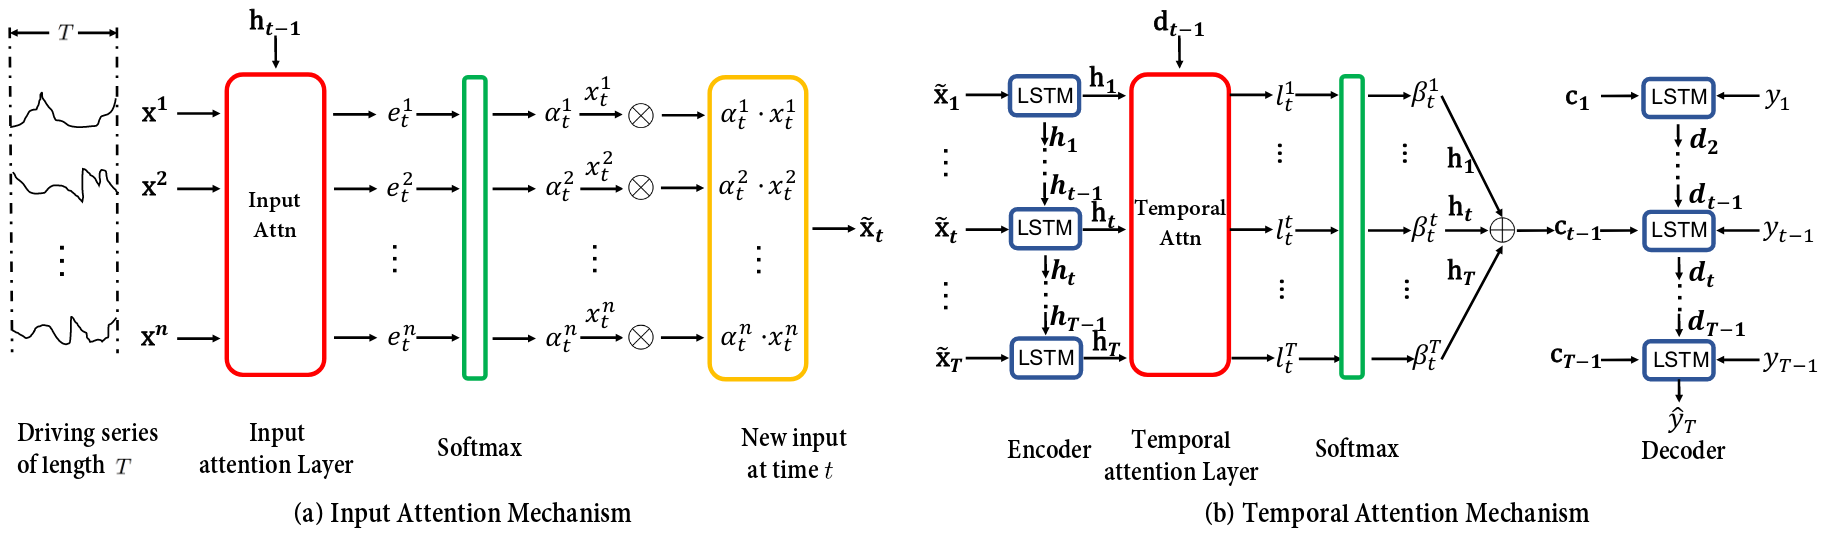
\includegraphics[width=\linewidth]{img/da-rnn.png} \\
\caption{DA-RNN model}
\label{fig:da-rnn}
\end{figure}


\paragraph{Multi-step-ahead encoder-decoder model}

In this paragraph we introduce a model for predicting more than a single value in 
the future using the same inputs of the single-step-ahead model. 
For the architecture we took inspiration from the original authors' comparison of
existing models and we extended the encoder-decoder model to predict the values
of multiple timesteps ahead for the target series.

For the encoder of this model we stacked two LSTM layers and collected only the 
final output as the set of the two hidden states and cell states. These vectors
represent the driving series.

For the decoder part we set as initial state of the decoder LSTM the output of the
encoder. We notice that the number of layers in the decoder is (and has to be) the
same as the encoder, as well as the dimension of the hidden sizes. We then give as
input to the decoder LSTM the vector containing the past history of the target 
series and we feed this vector to the cell at each time-step. The output hidden
state of the decoder is fed to a dense layer to obtain the final value for the 
desired timestep. The number of timesteps for the decoder is determined at test
time, that is we train the network to predict the value of the target series for
the next $k$ timesteps, however at test time we can ask the model to predict the 
next $k'$ timesteps with possibly $k' \ne k$.

\begin{figure}[ht]
\centering
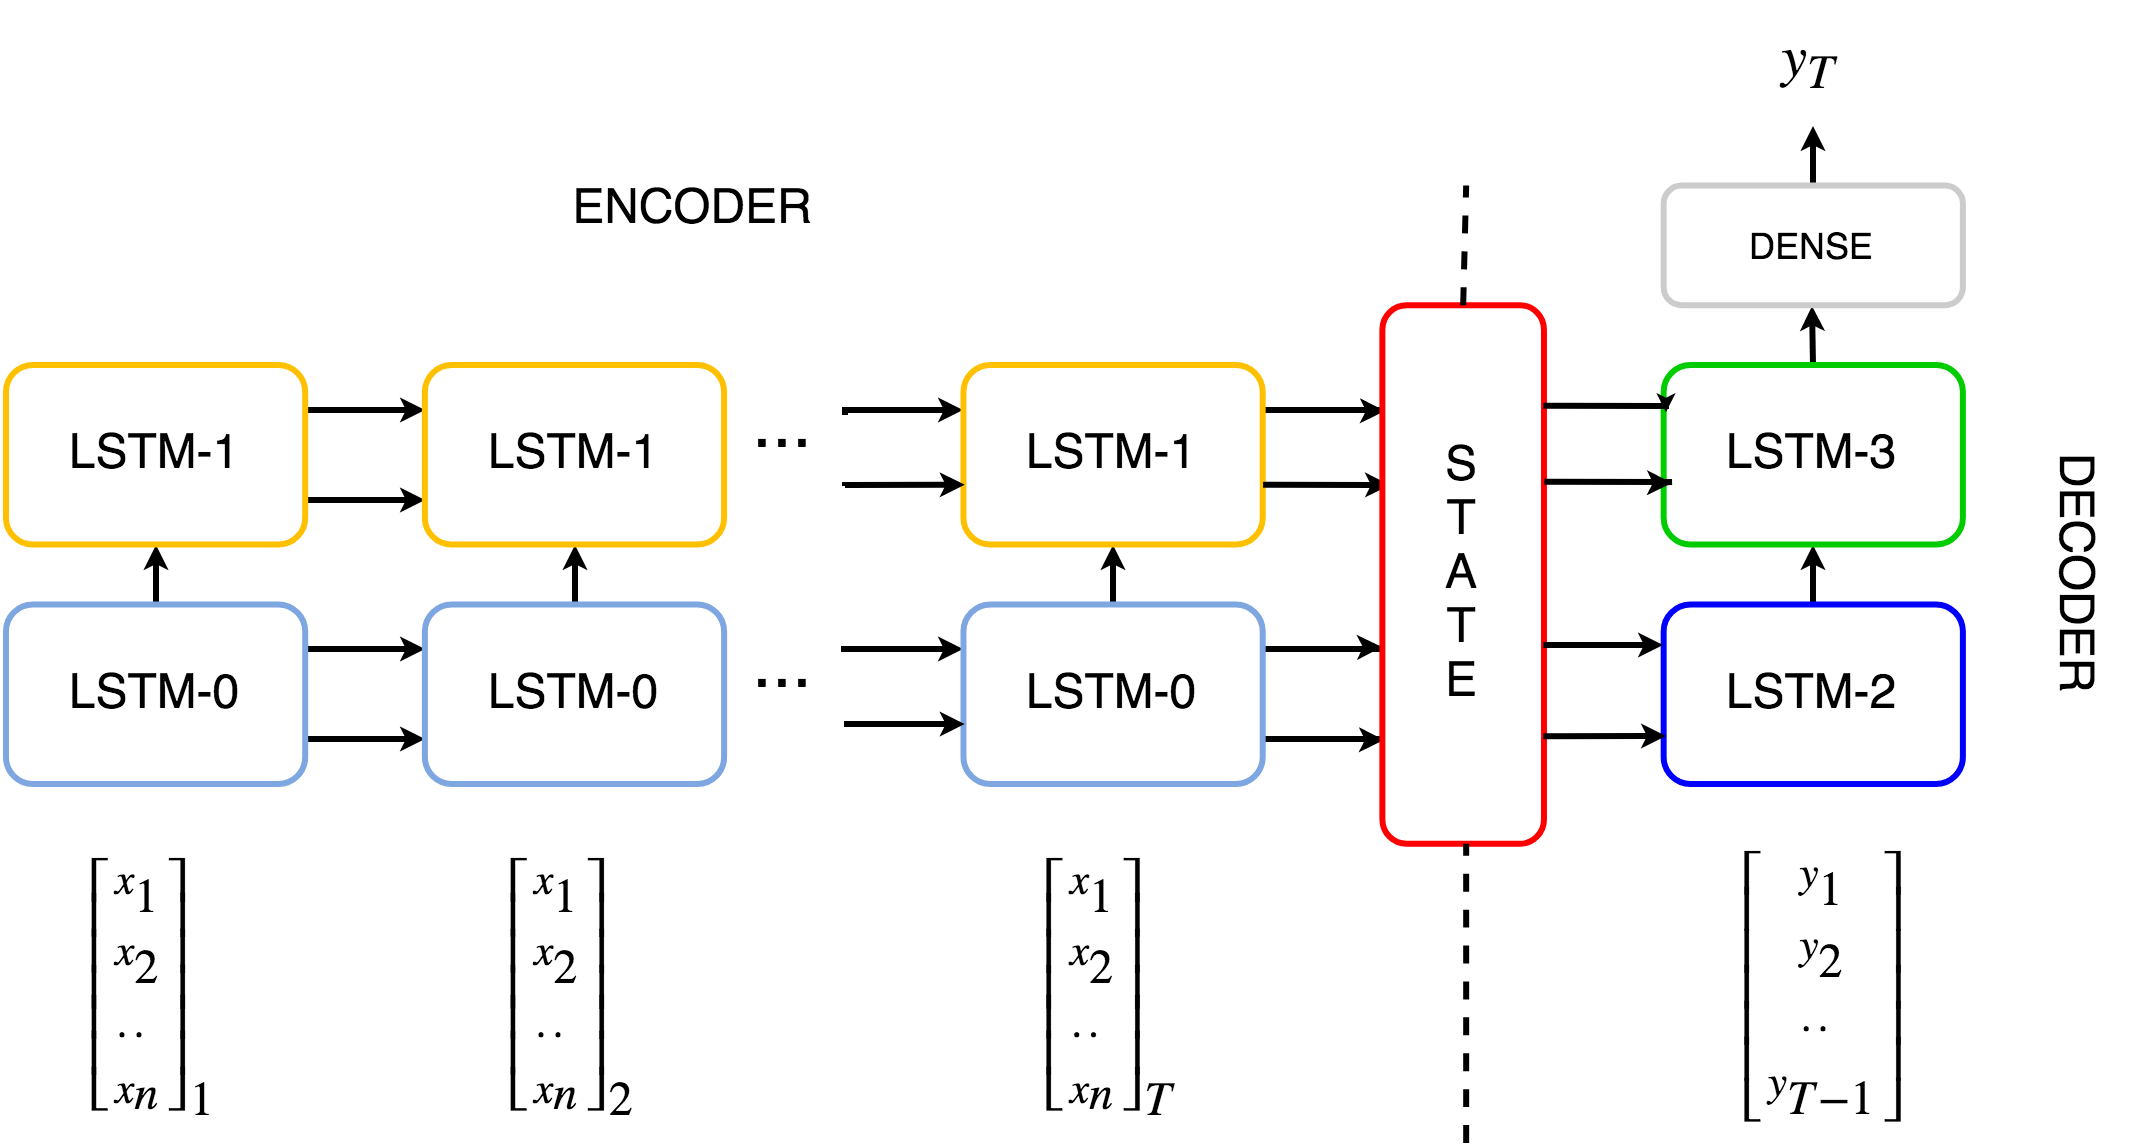
\includegraphics[width=0.7\linewidth]{img/ende-rnn.png} \\
\caption{Encoder Decoder model}
\label{fig:ende-rnn}
\end{figure}


\subsection{Implementation details}

\paragraph{DA-RNN implementation}

We used Tensorflow as the target framework to implement the model just
described. The reason for this choice is that we
could easily translate the equations of the model directly into the code and
define each step of the model without
trying to figure out the how to obtain the same results using the high level
APIs of Keras. This was because the
Keras documentation about RNNs to implement this custom attention model was a
bit foggy at the beginning so we decided
to step back to Tensorflow. 

For the encoder network we used the \texttt{LSTMCell} class from
\texttt{tensorflow.python.ops.rnn\_cell\_impl}.
We initially instantiated a zero state for the cell and the hidden states. Then
for each timestep we defined the
Tensorflow computational graph feeding the \texttt{LSTMCell} with the output of
the previous timestep combined with the
output of the attention. During this process we collect the output hidden
states of the cell for the various timesteps.
After the proper reshaping this output will be the input of the decoder network.

The decoder network implementation is very similar to the encoder also for the
attention part, the key difference where
the dimensions since the temporal attention works on a different range of
inputs. We initially defined weights and bias
variables for each operation of the attention mechanisms but we later made the
code more concise by using the
\texttt{tensorflow.layers.dense()} API.

In order to set the proper shapes in every part of the implementation of the
original model we used a nice facility of
Tensorflow called Eager Execution that allowed us to see the actual shapes of
variables at each step given a sample
input.

To make the experimentation modular we also defined a data class that loads all
the parameters and file paths from
JSON configuration files.

For the training procedure we use a standard back propagation algorithm since
the model is fully differentiable and we
set the mean squared error as the objective function. We selected the Adam
optimizer while for other parameters we
selected the best performing ones on the validation dataset as described in the
following section.

We used Tensorboard to graphically visualize the value of the loss across 
the training steps and the values of the evaluation metrics on the validation set 
at every epoch of training. Finally we also exploited the checkpointing facilities
offered by the framework to save two main set of values: the data needed to 
restart the training on a successive run of the training and the weights of the 
model that achieved the best performance in all the evaluation sessions. The final
tests indeed are done by loading the weights of the best model even if the 
training run for longer or later incurred in overfitting.

\paragraph{Encoder-decoder implementation}

For the encoder-decoder model we took advantage of the Keras, since we became more
familiar with its recurrent networks APIs. We instantiate a stacked 
\texttt{LSTMCell} and gave it as argument to a \texttt{RNN} layer. Using the 
functional API we applied this layer to the driving series' input and collected
the final state. The decoder is similar and we set it to return both states and 
sequences. We additionally set the initial state argument to the encoder output 
states. Finally we apply a \texttt{Dense} layer to the output with linear 
activation (since this is a regression problem).

We finally defined a callback in the \texttt{fit()} function call to make the
training stop if the value of the loss doesn't improve for a certain number of 
consecutive steps (the level of patience was empirically adjusted).

\section{Experiments}

We validated our implementation using the same set of metrics as the original 
authors and we performed some hyper-parameter tuning running the training with
different configuration files.

The metrics are the root mean squared error (RMSE), the mean absolute error (MAE) 
and finally the mean absolute percentage error (MAPE) which is scale-independent.

In order to obtain the better perfomance in the selected metrics we run
experiments under the following parameters values and obtain the following:

...

After we have obtained a good hyper-parameters set for the various models we 
compares their performance on our reference datasets. We obtained the following 
results:

...

In the following section we will also compare both qualitatively, i.e. visually 
analysing the predictions, and quantitatively with the metrics values the results 
of the DA-RNN model stripped of its basic components.


\section{Ablation Study}

To validate the usefulness and correctness of the dual-stage attention approach we
perform an ablation study of the model and report the values of the resulting 
three systems in the following tables. We notice that we here include the 
temporal-attention-only model together with the input-attention-only model that
was not evaluated in our original reference paper.

From the tables and pictures ...
we can see the effectiveness of the dual attention model with respect to the 
original simple encoder-decoder architecture. In particular you can notice on 
the graph reporting both the true and predicted curves that in correspondence 
with ... we have that ...

\section{Conclusion}

TODO

\section*{References}

\small

[1] Yao Qin, Dongjin Song, Haifeng Chen, Wei Cheng, Guofei Jiang, Garrison W.
Cottrell. A Dual-Stage Attention-Based Recurrent Neural Network for Time Series
Prediction. 2017.

\end{document}
